\question
Дана декартова система координат. Ось $x$ представляет собой множество $X$, ось $y$ - множество $Y$. На этих двух множествах определены бинарные отношения, которые схематически изображены в виде графиков выше (то есть, например, для графика с рис. 1 будет верно, что пары $(0, 0), (1, 1), (2, 2), (3, 3), (4, 4), (5, 5)$ входят в бинарное отношение, соответствующее графику). Для каждого из таких отношений определить:
\begin{itemize}
    \item Каким типом отношения соответствия оно является?
    \item Является ли оно функциональным отношением? Если да, то каким именно (сюръекция, инъекция, биекция)?
\end{itemize}
Обоснуйте своё решение. После этого, аналогично данным в условии графикам, придумайте отношение (любое), которое будет представлять собой полностью определенную функцию, и при этом будет инъективно и не сюръективно.
\\
\begin{figure}[h]

\begin{minipage}[h]{0.55\linewidth}
\end{minipage}
\begin{minipage}[h]{0.45\linewidth}
\center{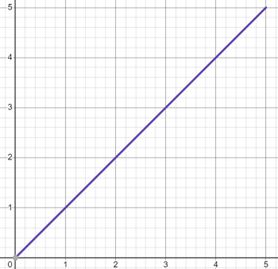
\includegraphics[width=0.7\textwidth]{pic/711.png}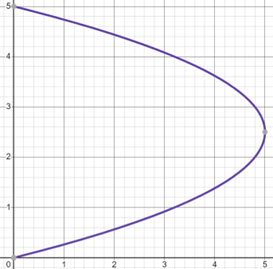
\includegraphics[width=0.7\textwidth]{pic/712.png}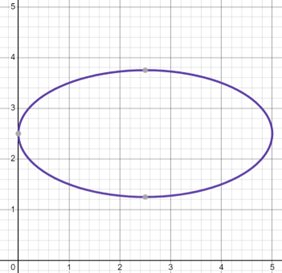
\includegraphics[width=0.7\textwidth]{pic/713.png} }
\end{minipage}
\end{figure}

---------------

Автор -- Тимур Гонтарь, М3206